\chapter{Diseño arquitectónico o de alto nivel}
\label{cap:disenoArquitectonico}

Este capítulo presenta el diseño arquitectónico de alto nivel del sistema \textbf{Taimotla}. Se definen las propiedades arquitectónicas objetivo, se representa la estructura física mediante un diagrama de despliegue, se describen sus componentes y se analizan las ventajas y limitaciones de la arquitectura propuesta.

%---------------------------------------------------------
\section{Propósito u objetivo de la arquitectura (en términos de propiedades)}
\label{sec:propositoArquitectura}

El propósito fundamental del diseño arquitectónico de \textbf{Taimotla} es dar cumplimiento a las siguientes propiedades de calidad del software:

\begin{itemize}
    \item \textbf{Seguridad y Privacidad:} El resguardo de los expedientes de NNA es crítico. La arquitectura debe garantizar que las peticiones se autentiquen y autoricen estrictamente en función del rol de usuario (Director, Coordinador o Especialista), impidiendo accesos no autorizados.
    \item \textbf{Concurrencia:} Permitir el acceso simultáneo de múltiples profesionales (médicos, abogados, psicólogos) consultando y editando información sobre el mismo o diferentes menores sin bloqueos o inconsistencias.
    \item \textbf{Desempeño y Velocidad:} Asegurar tiempos de respuesta bajos (menores a 1 segundo) en búsquedas dinámicas de expedientes y generación de catálogos mediante consultas SQL nativas altamente optimizadas.
    \item \textbf{Mantenibilidad:} Facilitar cambios o adiciones a los flujos operativos separando la lógica de presentación (plantillas HTML), la lógica de control (rutas Flask) y la lógica de acceso a datos (modelos SQL).
    \item \textbf{Simplicidad:} Minimizar el costo de infraestructura y la complejidad accidental de las herramientas, optando por una arquitectura Cliente-Servidor directa con psycopg2 nativo sin capas intermedias complejas.
\end{itemize}

%---------------------------------------------------------
\section{Diagrama arquitectónico}
\label{sec:diagramaArquitectura}

La distribución física y lógica de los componentes de la plataforma en su entorno de ejecución se detalla en el siguiente diagrama de despliegue:

\begin{figure}[htbp!]
\centering
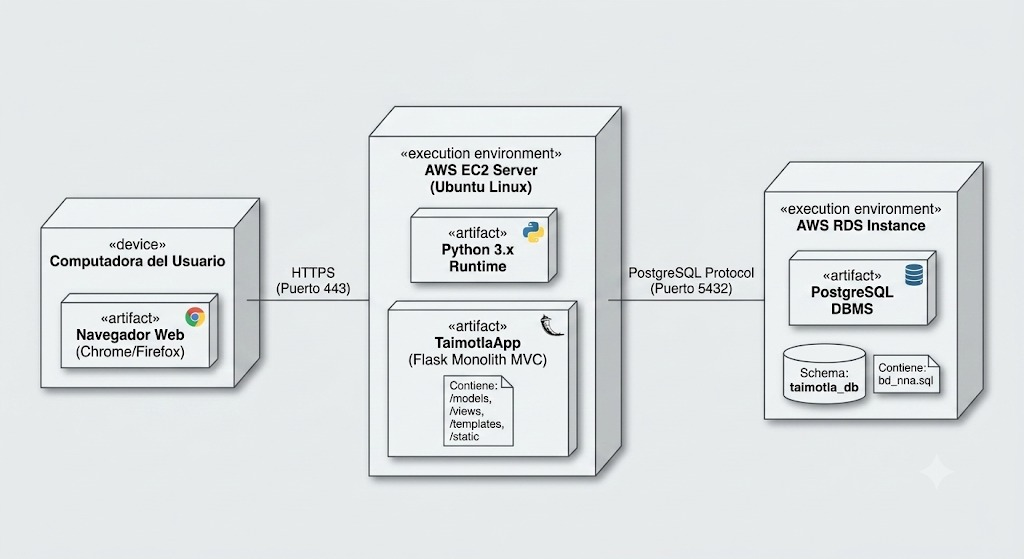
\includegraphics[width=0.75\textwidth]{CU/diagrama_de_despliegue.jpeg}
\caption{Diagrama de despliegue lógico y físico del sistema Taimotla.}
\label{fig:diagramaDespliegue}
\end{figure}

%---------------------------------------------------------
\section{Explicación (elementos, relaciones y reglas)}
\label{sec:explicacionArquitectura}

La arquitectura se compone de los siguientes elementos, relaciones y reglas operativas:

\subsection{Elementos (Nodos y Componentes)}
\begin{itemize}
    \item \textbf{Cliente Web (Navegador):} Dispositivo final del usuario. Renderiza las plantillas y ejecuta scripts de JavaScript ligero para validaciones rápidas en el navegador.
    \item \textbf{Servidor de Aplicación (Flask):} Centraliza la lógica de control. Recibe las peticiones HTTP, gestiona el estado de sesión del usuario (cifrada con la \texttt{SECRET\_KEY}) y enruta las solicitudes hacia los controladores correspondientes.
    \item \textbf{Servidor de Base de Datos (PostgreSQL):} Almacena de forma persistente e íntegra el esquema relacional con sus restricciones de integridad (llaves primarias y foráneas).
\end{itemize}

\subsection{Relaciones (Protocolos y Comunicación)}
\begin{itemize}
    \item \textbf{Cliente $\leftrightarrow$ Servidor:} Intercambio de peticiones y respuestas mediante el protocolo \textbf{HTTP/HTTPS}. Los formularios de datos son enviados en el cuerpo del método \texttt{POST}.
    \item \textbf{Servidor $\leftrightarrow$ Base de Datos:} Comunicación mediante el protocolo propietario de PostgreSQL utilizando el driver binario \textbf{psycopg2} bajo hilos de conexión seguros en el puerto 5432.
\end{itemize}

\subsection{Reglas Arquitectónicas}
\begin{itemize}
    \item \textbf{Desacoplamiento Estricto:} Ninguna plantilla (\texttt{templates/}) puede ejecutar consultas de base de datos directas. Todo acceso a datos se delega a las funciones definidas en \texttt{models/}.
    \item \textbf{Control de Transacciones:} Toda consulta SQL de modificación (\texttt{INSERT}, \texttt{UPDATE}, \texttt{DELETE}) debe ser controlada mediante el helper transaccional \texttt{get\_db\_cursor} para garantizar \texttt{commit} o \texttt{rollback} automático ante excepciones.
\end{itemize}

%---------------------------------------------------------
\section{Beneficios y limitaciones de la arquitectura (en términos de propiedades)}
\label{sec:beneficiosLimitaciones}

\subsection{Beneficios}
\begin{itemize}
    \item \textbf{Rendimiento Elevado (Performance):} Al utilizar consultas SQL parametrizadas directas sin la capa de abstracción de un ORM completo, las operaciones de inserción y búsquedas en la base de datos se ejecutan en milisegundos.
    \item \textbf{Bajo Consumo de Recursos (Simplicidad):} Flask es un microframework ligero, lo que reduce la memoria y procesamiento requeridos en el servidor en comparación con frameworks pesados.
    \item \textbf{Fácil Mantenibilidad (Maintainability):} La estricta separación de responsabilidades en carpetas facilita la depuración de errores.
\end{itemize}

\subsection{Limitaciones}
\begin{itemize}
    \item \textbf{Acoplamiento al Motor de Datos:} Al escribir sentencias SQL en dialecto nativo de PostgreSQL (ej. \texttt{serial}, \texttt{timestamp without time zone}), migrar el sistema a otro gestor (como MySQL u Oracle) requerirá reescribir consultas en los modelos.
    \item \textbf{Manejo de Conexiones Manual:} No se utiliza un Pool de conexiones avanzado por defecto, lo que limita la escalabilidad ante un número masivo de peticiones recurrentes (e.g. más de 500 usuarios simultáneos).
\end{itemize}
